\documentclass[11pt, a4paper]{article}

\usepackage{amssymb}
\usepackage{listings}
\usepackage[nodayofweek]{datetime}
\usepackage{setspace}
\usepackage{graphicx}
\usepackage{amsmath}
\usepackage[breaklinks]{hyperref}
\usepackage[all]{hypcap}

\setlength{\textheight}{8.63in}
\setlength{\textwidth}{5.9in}
\setlength{\topmargin}{-0.2in}
\setlength{\oddsidemargin}{0.3in}
\setlength{\evensidemargin}{0.3in}
\setlength{\headsep}{0.0in}

\setlength{\parindent}{0cm}
\setlength{\parskip}{0.4cm}

\begin{document}


\begin{titlepage}
\begin{center}
	\textsc{
			{\huge Generating Minimal Models}\\[0.2cm]
			{\large for}\\[0.3cm]
			{\huge Geometric Theories}
		}\\[1cm]
	A Major Qualifying Project Report\\
	submitted to the Faculty of\\[0.7cm]
	\textsc{ \large Worcester Polytechnic Institute }\\[0.7cm]
	in partial fulfillment of\\
	the requirements for the degree of\\
	Bachelor of Science\\[1cm]
	by\\[1cm]
	~\hspace{2cm}\dotfill\hspace{2cm}~\\
	\textsc{\Large Michael Ficarra}\\[1cm]
	on\\[1cm]
	{\Large \today}\\
	\vfill
	\begin{flushright}
		\hspace{8cm}\dotfill \\
		\textsc{Daniel Dougherty}\\
		professor, project advisor\\
	\end{flushright}
\end{center}
\end{titlepage}


\pagenumbering{roman}

~\\
\vfill
\begin{abstract}
This paper describes a method, referred to as the chase, for generating jointly
minimal models for a geometric theory. A minimal model for a theory is a model
for which there exists a homomorphism to any other model that can satisfy the
theory. These models are useful in solutions to problems in many practical
applications, including but not limited to firewall configuration examination,
protocol analysis, and access control evaluation. Also described is a Haskell
implementation of the chase and its development process and design decisions.
\end{abstract}
\vfill
~\\
\newpage

\renewcommand{\contentsname}{Table of Contents}
\tableofcontents \newpage
%\listoffigures \newpage
%\listoftables \newpage

\pagenumbering{arabic}


%\onehalfspacing

% main paper sections
\section{Introduction}

	\textbf{ remove this? }

	This document details work done for a Major Qualifying Project at Worcester
	Polytechnic Institute by Michael Ficarra in partial fulfillment of the
	requirements for a Bachelor of Science degree in Computer Science.

	Section \ref{sec:technical_background} can be used as a reference for terms
	discussed in later sections. Appendices \ref{sec:appendix_glossary} and
	\ref{appendix_syntax_table} contain a glossary and syntax reference,
	respectively.

	\subsection{Goals}

		The two main goals of this Major Qualifying Project are:

		\begin{enumerate}
		\item to implement an algorithm known as ``the chase" accurately
		and with a well-defined, usable interface, and
		\item to use the chase implementation for a real-world
		application: generating models used in analysis of a specific protocol
		\end{enumerate}

		Secondary goals include implementing various optimizations and
		integrating the chase implementation into a program that can take
		advantage of the functionality it provides.

	\subsection{The Chase}

		\textbf{ this whole section needs some expanding still }

		\emph{The chase} is an algorithm used to find jointly minimal models
		(see \ref{sec:technical_background.minimal_models}) for a set of
		geometric logic formul{\ae}. Many common real-world problems can be
		expressed as a set of geometric logic formul{\ae} (see
		\ref{sec:technical_background.geometric_logic}). When these problems
		have an unbounded scope of possible solutions, the chase can be used to
		find the possible solutions that are interesting. This allows
		researchers to go through only models that represent a large set of
		models rather than testing each of the infinite number of models
		separately.

		To generate these jointly minimal models, the chase begins with a model
		$\mathbb{M}$ that has an empty domain and no facts. The chase goes
		through each formula $\sigma$ in the geometric theory $T$ such that
		$\mathbb{M} \not\models \sigma$ and alters $\mathbb{M}$ so that
		$\mathbb{M} \models \sigma$. Geometric formul{\ae} are implications of
		positive-existential formul{\ae} (see
		\ref{sec:technical_background.geometric_logic}). Positive-existential
		formul{\ae} have the useful property in that adding elements/facts to a
		model that satisfies one will never cause the model to no longer
		satisfy that formula. Because of this, the chase can keep adding to the
		model until all formul{\ae} are satisfied. The set of all models
		generated by this process is a jointly minimal set for the input theory
		$T$.

		The chase is nondeterministic over disjunctions. When a disjunction is
		encountered, a disjunct is chosen and the chase continues until it
		encounters another disjunct.

	\subsection{Chase Implementation}

		We will see in section \ref{sec:implementation} that, in a Haskell
		implementation of the chase, both disjuncts can be satisfied by forking
		the chase and returning a list containing the concatenation of the
		lists returned by the forks. In this way, we can deterministically
		calculate a set of jointly minimal models by using a naturally
		nondeterministic algorithm.

	\subsection{Application}

		Cryptographic protocol analysis is the particular application that is
		explored in section \ref{sec:application.strand_spaces}. In this
		application, protocols are modeled in the strand space formalism. Each
		role of every participant in a legal run of the protocol is modeled as
		a strand. The roles of a special participant that does not obey the
		rules of the protocol are called adversary strands (see
		\ref{sec:application.the_adversary}). These adversary strands consist
		of a series of nodes that send/receive messages to/from regular strands
		while manipulating those messages. Because the positions and actions of
		adversary strands are variable, there exists a large number of possible
		runs of a single protocol. It is prohibitive to test all of these to
		find if they break assumptions made about the properties of the
		protocol. The runs of this protocol can be represented as a geometric
		theory and passed to the chase to find minimal models. When minimal
		models are found, they can describe nearly all interesting ways that
		the adversaries can interact with regular strands. These models can
		then be analysed in a finite amount of time.

\section{Technical Background}
\label{sec:technical_background}

	\subsection{Vocabulary}

		A \emph{relation symbol}, often called a \emph{predicate}, can be any
		unique symbol. An \emph{arity} function takes a relation symbol as
		input and returns a non-negative integer. A \emph{vocabulary} is a
		construct containing a set of relation symbols and an arity function.

	\subsection{Models}

		A \emph{model} $\mathbb{M}$ for a vocabulary $\mathcal{V}$ is a
		construct that consists of:
		\begin{itemize}
		\item a set, denoted $|\mathbb{M}|$, called the \emph{universe} or \emph{domain} of $\mathbb{M}$
		\item for each pairing of a predicate $R$ of arity $k$ in $\mathcal{V}$, a relation $R^\mathbb{M}_k \subseteq |\mathbb{M}|$
		\end{itemize}
		The relation itself is a set of tuples of members from the universe.

		\begin{definition}
			Let $\mathbb{A}$ and $\mathbb{B}$ be models. $\mathbb{A}$ is a
			\emph{submodel} of $\mathbb{B}$ if
			\begin{itemize}
			\item $|\mathbb{A}| \subseteq |\mathbb{B}|$
			\item for each relation $R$, $R^\mathbb{A} \subseteq R^\mathbb{B}$

			That is, for each tuple $\vec a$ from $|\mathbb{A}|$, $\vec a \in
			R^\mathbb{A}$ implies  $\vec a \in R^\mathbb{B}$.
			\end{itemize}
		\end{definition}

	\subsection{First-order Logic}

		\emph{First-order logic}, also called \emph{predicate logic}, is a
		formal logic system. A first-order logic formula is defined inductively
		by the following:
		\begin{itemize}
		\item if $R$ is a relation symbol of arity $k$ and each of $x_0 \ldots x_{k-1} \in \vec{x}$ is a variable, then $R(\vec{x})$ is a formula, specifically an \emph{atomic formula}
		\item if $x$ and $y$ are variables, then $x = y$ is a formula
		\item $\top$ and $\bot$ are formul{\ae}
		\item if $\alpha$ is a formula, then $(\neg\alpha)$ is a formula
		\item if $\alpha$ and $\beta$ are formul{\ae}, then $(\alpha \wedge \beta)$ is a formula
		\item if $\alpha$ and $\beta$ are formul{\ae}, then $(\alpha \vee \beta)$ is a formula
		\item if $\alpha$ and $\beta$ are formul{\ae}, then $(\alpha \to \beta)$ is a formula
		\item if $\alpha$ is a formula and $x$ is a variable, then $(\forall\ x : \alpha)$ is a formula
		\item if $\alpha$ is a formula and $x$ is a variable, then $(\exists\ x : \alpha)$ is a formula
		\end{itemize}

		For our purposes, this logic system will not contain any constant
		symbols or function symbols which are commonly included in first-order
		logic. We will see in section
		\ref{sec:technical_background.geometric_logic} that these are
		unnecessary and can be replicated using other, allowed constructs.

		A shorthand notation may sometimes be used which omits either the left
		or right side of an implication and denotes ($\top \to \sigma$) and
		($\sigma \to \bot$) respectively. If $\alpha$ is a formula and
		$\vec{x}$ is a set of variables of size $k$, then $(\forall\ \vec{x} :
		\alpha)$ is $(\forall\ x_0 \ldots \forall\ x_{k-1} : \alpha)$. If
		$\alpha$ is a formula and $\vec{x}$ is a set of variables of size $k$,
		then $(\exists\ \vec{x} : \alpha)$ is $(\exists\ x_0 \ldots \exists\
		x_{k-1} : \alpha)$.

	\subsection{Variable Binding}

		The set of free variables in a formula $\sigma$, denoted $free(\sigma)$
		is defined inductively as follows:
		\begin{itemize}
		\item $free( R(x_0,\ldots,x_n) )$ = $\{x_0,\ldots,x_n\}$
		\item $free(\top)$ = $\emptyset$
		\item $free(\bot)$ = $\emptyset$
		\item $free(x = y)$ = $\{x,y\}$
		\item $free(\neg\alpha)$ = $free(\alpha)$
		\item $free(\alpha \wedge \beta)$ = $free(\alpha) \cup free(\beta)$
		\item $free(\alpha \vee   \beta)$ = $free(\alpha) \cup free(\beta)$
		\item $free(\alpha \to    \beta)$ = $free(\alpha) \cup free(\beta)$
		\item $free(\forall\ x : \alpha)$ = $free(\alpha)\ \backslash\ \{x\}$
		\item $free(\exists\ x : \alpha)$ = $free(\alpha)\ \backslash\ \{x\}$
		\end{itemize}
		A formula $\sigma$ is a \emph{sentence} if $free(\sigma) = \emptyset$.

	\subsection{Environment}

		An \emph{environment} $\lambda$ for a model $\mathbb{M}$ is a function
		from a set of variables $\vec v$ to $|\mathbb{M}|$. The syntax
		$\lambda_{[v \mapsto a]}$ denotes the environment $\lambda'(x)$ that
		returns $a$ when $x=v$ and returns $\lambda(x)$ otherwise.

	\subsection{Satisfiability}

		A model $\mathbb{M}$ is said to satisfy a formula $\sigma$ in an
		environment $\lambda$, denoted $\mathbb{M} \models_\lambda \sigma$ and
		read ``under $\lambda$, $\sigma$ is true in $\mathbb{M}$", when
		\begin{itemize}
		\item $\sigma$ is a relation symbol $R$ and $R(\lambda(a_0) , \ldots , \lambda(a_n)) \in \mathbb{M}$ where $a$ is a set of variables
		\item $\sigma$ is of the form $\neg\alpha$ and $\mathbb{M} \not\models_\lambda \alpha$
		\item $\sigma$ is of the form $\alpha\wedge\beta$ and both $\mathbb{M} \models_\lambda \alpha$ and $\mathbb{M} \models_\lambda \beta$
		\item $\sigma$ is of the form $\alpha\vee\beta$ and either $\mathbb{M} \models_\lambda \alpha$ or $\mathbb{M} \models_\lambda \beta$
		\item $\sigma$ is of the form $\alpha\to\beta$ and either $\mathbb{M} \not\models_\lambda \alpha$ or $\mathbb{M} \models_\lambda \beta$
		\item $\sigma$ is of the form $\forall\ x : \alpha$  and for every $x' \in |\mathbb{M}|$, $\mathbb{M} \models_{\lambda[x \mapsto x']} \alpha$
		\item $\sigma$ is of the form $\exists\ x : \alpha$  and for at least one $x' \in |\mathbb{M}|$, $\mathbb{M} \models_{\lambda[x \mapsto x']} \alpha$
		\end{itemize}
		The notation $\mathbb{M} \models \sigma$ (no environment specification)
		means that, under the empty environment $l$, $\mathbb{M} \models_l \sigma$.

		A model $\mathbb{M}$ satisfies a set of formul{\ae} $\Sigma$ under an
		environment $\lambda$ if for every $\sigma$ such that $\sigma \in
		\Sigma$, $\mathbb{M} \models_\lambda \sigma$. This is denoted as
		$\mathbb{M} \models_\lambda \Sigma$ and read ``$\mathbb{M}$ is a model
		of $\Sigma$".

	\subsection{Entailment}

		Given an environment $\lambda$, a set of formul{\ae} $\Sigma$ is said
		to \emph{entail} a formula $\sigma$ ($\Sigma \models_\lambda \sigma$)
		if the set of all models satisfied by $\Sigma$ under $\lambda$ is a
		subset of the set of all models satisfying $\sigma$ under $\lambda$.
		In other words, given a model $\mathbb{M}$, a set of formul{\ae}
		$\Sigma$, and a formula $\sigma$ such that $\Sigma \models \sigma$,
		whenever $\mathbb{M} \models \Sigma$, $\mathbb{M} \models \sigma$.

		The notation used for satisfiability and entailment is very similar, in
		that the operator used ($\models$) is the same, but they can be
		distinguished by the type of left operand.

	\subsection{Homomorphisms}

		A \emph{homomorphism from $\mathbb{A}$ to $\mathbb{B}$} is a function
		$h: |\mathbb{A}|\to|\mathbb{B}|$ such that, for each relation symbol
		$R$ and tuple $\langle a_0 , \ldots , a_n \rangle$, $\langle a_0 ,
		\ldots , a_n  \rangle \in R^\mathbb{A}$ implies $\langle h(a_0) ,
		\ldots , h(a_n) \rangle \in R^\mathbb{B}$. The identity function is a
		homomorphism from any model $\mathbb{M}$ to itself.

		%\begin{theorem}
		%	A homorphism $h: |\mathbb{M}| \to |\mathbb{N}|$
		%	is a composition of zero or more of the following functions:
		%	\begin{itemize}
		%	\item $addDomain(\omega):
		%		|\mathbb{M}| \to |\mathbb{M}| \cup \vec\omega$ where
		%		$\vec\omega$ is non-empty and each $\omega \in \vec\omega$ is a
		%		domain member not in $|\mathbb{M}|$
		%	\item $addFact:
		%		\mathbb{M} \to \mathbb{N}$ where $|\mathbb{M}| = |\mathbb{N}|$,
		%		for each fact $R^\mathbb{M}(\alpha_0,\ldots,\alpha_n)$, there
		%		exists an $R^\mathbb{N}(\alpha_0,\ldots,\alpha_n)$, and for
		%		each predicate $P \in \mathbb{N}$ there exists one or more
		%		facts $P^\mathbb{N}(\gamma_0,\ldots,\gamma_k)$
		%	\item $rename:
		%		\mathbb{M} \to \mathbb{N}$ where, for every
		%		$R^\mathbb{M}(\alpha_0,\ldots,\alpha_n)$ where $\alpha \in
		%		|\mathbb{M}|$, there exists an
		%		$R^\mathbb{N}(\eta(\alpha_0),\ldots,\eta(\alpha_n))$ where
		%		$\eta$ is a homomorphism
		%	\end{itemize}
		%\end{theorem}

		A homomorphism $h$ is also a \emph{strong homomorphism} if, for each
		relation symbol $R$ and tuple $\langle a_0 , \ldots , a_n \rangle$,
		$\langle a_0 , \ldots , a_n  \rangle \in R^\mathbb{A}$ if and only if
		$\langle h(a_0) , \ldots , h(a_n) \rangle \in R^\mathbb{B}$.

		The notation $\mathbb{M} \preceq \mathbb{N}$ means that there exists a
		homomorphism $h : \mathbb{M} \to \mathbb{N}$. $\preceq$ has the
		property that $\mathbb{A} \preceq \mathbb{B} \wedge \mathbb{B} \preceq
		\mathbb{C}$ implies $\mathbb{A} \preceq \mathbb{C}$. However,
		$\mathbb{M} \preceq \mathbb{N} \wedge \mathbb{N} \preceq \mathbb{M}$
		does not imply that $\mathbb{M} = \mathbb{N}$. For example, fix two
		models $\mathbb{M}$ and $\mathbb{N}$ that are equivalent except that
		$|\mathbb{N}| = |\mathbb{M}| \cup \omega$ where $\omega \not\in
		|\mathbb{M}|$. Both $\mathbb{M} \preceq \mathbb{N}$ and $\mathbb{N}
		\preceq \mathbb{M}$ are true, yet $\mathbb{M} \neq \mathbb{N}$.

		Given two models $\mathbb{M}$ and $\mathbb{N}$, when $\mathbb{M}
		\preceq \mathbb{N}$ and $\mathbb{N} \preceq \mathbb{M}$, $\mathbb{M}$
		and $\mathbb{N}$ are \emph{homomorphically equivalent}. Homomorphic
		equivalence between a model $\mathbb{M}$ and a model $\mathbb{N}$ is
		denoted $\mathbb{M} \simeq \mathbb{N}$.

		Given models $\mathbb{M}$ and $\mathbb{N}$ where $\mathbb{M} \preceq
		\mathbb{N}$ and a formula in positive-existential form $\sigma$, if
		$\mathbb{M} \models \sigma$ then $\mathbb{N} \models \sigma$.

		A homomorphism $h : \mathbb{A} \to \mathbb{B}$ is also an
		\emph{isomorphism} when $h$ is 1:1 and onto and the inverse function
		$h^{-1} : \mathbb{B} \to \mathbb{A}$ is a homomorphism.

	\subsection{Universal Models}
	\label{sec:technical_background.universal_models}

		\emph{Universal models}, also called \emph{universal} models, are models
		for a theory $\mathcal{T}$ with the special property that there exists a
		homomorphism from the universal model to any other model that satisfies
		$\mathcal{T}$. Intuitively, universal models have no unnecessary entities or
		relations and thus display the least amount of constraint necessary to
		satisfy the theory for which they are universal. Any model to which there
		exists a homomorphism from a universal model will have more constraints
		than the universal model.

		A set of models $\mathcal{M}$ is said to be \emph{jointly universal} for
		a set of formul{\ae} $\Sigma$ when, for every model $\mathbb{N}$ such
		that $\mathbb{N} \models \Sigma$, there exists a homomorphism from a
		model $\mathbb{M} \in \mathcal{M}$ to $\mathbb{N}$. It follows that any
		superset of a jointly universal set of models is also jointly universal.

		More than one universal model may exist for a given theory. Given a model
		$\mathbb{M}$ that is universal for a theory $\mathcal{T}$, any model $\mathbb{N}$
		such that $\mathbb{N} \simeq \mathbb{M}$ is also universal for $\mathcal{T}$.

		Not every theory must have a universal model. A simple example of this is
		the theory containing a single formula $\sigma$ where $\sigma$ contains
		a disjunction. There exists no single universal model for the formula $P
		\vee Q$ ($P$ and $Q$ are relations with arity $0$) because any model that
		satisfies both $P$ and $Q$ would not have a homomorphism to a model
		that satisfies the theory with only $P$ or $Q$ in its set of facts.
		However, the set containing a model $\mathbb{M}$ that contains $P$ in
		its set of facts and a model $\mathbb{N}$ that contains $Q$ in its
		set of fact would be \emph{jointly} universal.

	\subsection{Positive Existential Form}

		Formul{\ae} in \emph{positive existential form} are constructed using
		only conjunctions ($\wedge$), disjunctions ($\vee$), existential
		quantifications ($\exists$), tautologies ($\top$), contradictions
		($\bot$), equalities, and relations.

		\begin{theorem}
			\label{pef_theorem}
			The set of models of a sentence $\sigma$ is closed under homomorphisms
			if and only if $\sigma$ is logically equivalent to a positive
			existential formula $\varphi$.
		\end{theorem}

		\begin{proof}
			This is a well-known classical result in model theory. See
			\cite{ChangKeisler73}, section 5.2 for example.

			We will only use one direction of Theorem \ref{pef_theorem}: the
			fact that if a sentence is in positive-existential form then it is
			closed under homomorphisms. To keep this paper self-contained, we
			provide here a proof of this fact.

			It suffices to prove the following, more general, claim for
			positive-existential \emph{formul{\ae}}.

			\begin{quote}
				If $\sigma$ is a positive-existential formula, $\mathbb{M}$ is
				a model, $\lambda : [var] \to |\mathbb{M}|$ is an environment
				such that $\mathbb{M} \models_\lambda \sigma$, and $h$ is a
				homomorphism $h : |\mathbb{M}| \to |\mathbb{M}'|$, then
				$\mathbb{M}' \models_{h\circ\lambda} \sigma$.
			\end{quote}

			We prove this by induction over formul{\ae}.

			When $\sigma$ is an atomic formula $R(x_0,\ldots,x_n)$, we know
			that $R(\lambda(x_0),\ldots,\lambda(x_n)) \in \mathbb{M}$ and by
			the definition of a homomorphism
				\[
				R((h(\lambda(x_0)),\ldots,(h(\lambda(x_n))) \in \mathbb{M}'
				\]
			That is,
				\[
				R((h\circ\lambda)(x_0),\ldots,(h\circ\lambda)(x_n)) \in \mathbb{M'}
				\]
			as desired.

			When $\sigma$ is $x=y$, we know that $\lambda(x) = \lambda(y)$, so
			$h(\lambda(x))$ must be $h(\lambda(y))$.

			When $\sigma$ is $\bot$, there exists no $\lambda$ such that
			$\mathbb{M} \models_\lambda \bot$, so the hypothesis of our claim
			never holds, which causes our claim to always hold.

			When $\sigma$ is $\top$, we know that $\mathbb{M} \models_\lambda
			\top$ and by the induction hypothesis, $\mathbb{M}'
			\models_{h\circ\lambda} \top$.

			When $\sigma$ is $\alpha \wedge \beta$, we know that $\mathbb{M}
			\models_\lambda \alpha$ and by the induction hypothesis
			$\mathbb{M}' \models_{h\circ\lambda} \alpha$. We also know that
			$\mathbb{M} \models_\lambda \beta$ and by the induction hypothesis
			$\mathbb{M}' \models_{h\circ\lambda} \beta$. By the definition of
			conjunction, because $\mathbb{M}' \models_{h\circ\lambda} \alpha$
			and $\mathbb{M}' \models_{h\circ\lambda} \beta$, we know that
			$\mathbb{M}' \models_{h\circ\lambda} \alpha \wedge \beta$.

			When $\sigma$ is $\alpha \vee \beta$, we know that if $\mathbb{M}
			\models_\lambda \alpha$, by the induction hypothesis $\mathbb{M}'
			\models_{h\circ\lambda} \alpha$. We also know that if $\mathbb{M}
			\models_\lambda \beta$, by the induction hypothesis $\mathbb{M}'
			\models_{h\circ\lambda} \beta$. By the definition of disjunction,
			because $\mathbb{M}' \models_{h\circ\lambda} \alpha$ or
			$\mathbb{M}' \models_{h\circ\lambda} \beta$, we know that
			$\mathbb{M}' \models_{h\circ\lambda} \alpha \vee \beta$.

			When $\sigma$ is $\exists\ \vec x : \alpha$, we know that
			$\mathbb{M} \models_\lambda \exists\ x : \alpha$, and want to prove
			that $\mathbb{M}' \models_{h\circ\lambda} \exists\ x : \alpha$.
			There is a $d \in |\mathbb{M}|$ such that $\mathbb{M}
			\models_{\lambda[x\mapsto d]} \alpha$. By our induction
			hypothesis, $\mathbb{M}' \models_{h\circ(\lambda[x\mapsto d])}
			\alpha$. This is equivalent to $\mathbb{M}'
			\models_{(h\circ\lambda)[x\mapsto h(d)]} \alpha$.
		\end{proof}

		\begin{corollary}
			If $\mathbb{M}$ is a submodel of $\mathbb{N}$, $\sigma$ is a
			positive-existential formula, and $\mathbb{M} \models \sigma$, then
			$\mathbb{N} \models \sigma$.
		\end{corollary}

		\begin{proof}
			If $\mathbb{M}$ is a submodel of $\mathbb{N}$ the inclusion
			function from $\mathbb{M}$ to $\mathbb{N}$ is a homomorphism.
		\end{proof}

	\subsection{Geometric Logic}
	\label{sec:technical_background.geometric_logic}

		\emph{Geometric logic} formul{\ae} are implicitly universally
		quantified implications between positive existential formul{\ae}. More
		specifically, a geometric logic formula is of the form
			\[
			\forall\ \vec{x} : F_L \to F_R
			\]
		where $\vec{x} = free(F_L) \cup free(F_R)$, $free$ is the function that
		returns the set of all free variables for a given formula, and both
		$F_L$ and $F_R$ are first-order logic formul{\ae} in positive
		existential form.

		A set of geometric logic formul{\ae} is called a \emph{geometric
		theory}.

		It is convention to treat a positive existential formula $\sigma$ as
		$\top \to \sigma$ when expecting a geometric logic formula. It is also
		convention to treat a negated positive existential formula $\neg\sigma$
		as $\sigma \to \bot$.


		\subsubsection{Examples}
		\label{sec:technical_background.geometric_logic.examples}

			\begin{enumerate}
			\item
			We can express properties of an ordering relation $R$:
			\begin{eqnarray*}
			reflexivity   & \quad & \top \to R(x,x)                  \\
			symmetry      & \quad & R(x,y) \to R(y,x)                \\
			asymmetry     & \quad & R(x,y) \wedge R(y,x) \to \bot    \\
			serial        & \quad & \top \to \exists\ y : R(x,y)     \\
			totality      & \quad & \top \to R(x,y) \vee R(y,x)      \\
			transitivity  & \quad & R(x,y) \wedge R(y,z) \to R(x,z)
			\end{eqnarray*}

			\item \label{simulate_equality}
			Equality can be encoded as the two relations
				\begin{eqnarray*}
				EQ(x,y)                & \to & EQ(y,x)  \\
				EQ(x,y) \wedge EQ(y,z) & \to & EQ(x,z)
				\end{eqnarray*}
			along with, for each relation symbol $P$ in the vocabulary and each
			of its variables $\vec x$, a relation of the form $P(x_0) \wedge
			EQ(x_0,z) \to P(z)$. For example, the relation $P$ with arity $2$
			would require the following rules.
				\begin{eqnarray*}
				P(x,y) \wedge EQ(x,z) & \to & P(z,y)  \\
				P(x,y) \wedge EQ(y,z) & \to & P(x,z)
				\end{eqnarray*}

			This is sometimes convenient because it allows one to define a
			logic system that does not include equality without limiting
			the expressiveness of the system.

			\item
			Negation of a relation $R$ with arity $k$ can be used in
			positive-existential formul{\ae} by introducing another relation
			$R'$ with arity $k$, adding two formul{\ae} of the form
				\begin{eqnarray*}
				R \wedge R' & \to & \bot       \\
				\top        & \to & R \vee R'
				\end{eqnarray*}
			and using $R'$ where $\neg R$ would be used.

			\item
			Relations with an arity of zero will behave like constant symbols.
			For example, the constant $C$ can be represented by the relation
			$C()$.

			\item
			A binary relation $F(x,y)$ will behave like a function when
			expressed using the geometric logic formul{\ae}
			\begin{eqnarray}
			\label{function1}
				{}                   & \to & \exists\ y : F(x,y)  \\
			\label{function2}
				F(x,y) \wedge F(x,z) & \to & y = z
			\end{eqnarray}
			If \eqref{function1} is omitted, $F$ behaves like a partial
			function instead.
			\end{enumerate}

\section{The Chase}
\label{sec:chase}

	The \emph{chase} is a function that, when given a geometric theory, will
	generate a model in the set of jointly universal models for that theory. More
	specifically, if $\mathcal{U}$ is the set of all models obtained from an
	execution of the chase over a geometric theory $T$, for any model
	$\mathbb{M}$ such that $\mathbb{M} \models T$, there is a homomorphism from
	some model $\mathbb{U} \in \mathcal{U}$ to $\mathbb{M}$. Note that given a
	model $\mathbb{M}$ returned by the chase there may exist a model
	$\mathbb{N}$ such that $\mathbb{N} \preceq \mathbb{M}$.

	Verifying the universality of a model or the joint universality of a set of
	models requires checking if a homomorphism exists from the universal model(s)
	to each of the infinite set of all models that satisfy the theory. It may
	not at first seem obvious that generating a universal model would be a
	computable task, but it will be shown that the chase is able to do this,
	and it will be proven that the models it returns during successful runs are
	in fact members of a set of jointly universal models.

	Geometric logic formul{\ae} are used by the chase both because they are
	natural expressions of many common applications and because they take
	advantage of the useful properties of the positive-existential formul{\ae}
	of which they are constructed. Recall that, when adding any relations or
	domain members to a model that satisfies a positive-existential formula,
	the model will always satisfy the formula. This is particularly helpful
	when trying to create a model that satisfies all formul{\ae} in a geometric
	theory.

	\textbf{ I should probably talk about fairness here, I'm just not exactly sure where }

	\subsection{Algorithm}
	\label{sec:chase.algorithm}

		The chase starts with an input theory $T$ and a model $\mathbb{M}$ that
		has an empty domain and an empty set of facts.

		\textbf{ I need this thoroughly checked for correctness }

		\begin{algorithm}[H]
		\DontPrintSemicolon
		\TitleOfAlgo{The Chase}
		\While{$\exists$ a formula $\sigma \in T$ and an environment $\lambda$ such that $\mathbb{M} \not\models_\lambda \sigma$}{
			let $\sigma$ be $\alpha \to \beta$ \;
			\lIf{$\beta = \bot$}{
				halt with a failure \;
			}
			\lIf{$\beta$ contains a disjunction}{
				choose a disjunct $\delta$ and redefine $\beta$ as $\delta$ \;
			}
			\ForAll{variables $v \in free(\beta)$ for which $\lambda$ is undefined}{
				add a new domain member $\omega$ such that $\omega \not\in |\mathbb{M}|$ to $|\mathbb{M}|$ \;
				redefine $\lambda$ as $\lambda_{v \mapsto \omega}$ \;
			}
			\ForAll{relations $R(\alpha_0,\ldots,\alpha_n) \in \mathbb{M}$}{
				replace each variable $\alpha_i \in \{\alpha_0,\ldots,\alpha_n\}$ with $\lambda(\alpha_i)$ \;
			}
		}
		halt with result $\mathbb{M}$ \;
		\end{algorithm}

		\textbf{Is what I have only applicable to a $\beta$ that is a single
		atomic? Do I have to recursively call $chase$ or call a helper for
		conjunctions and handle equality like I do in the implementation?
		Modify $\lambda$ for existential quantifiers like in the implementation
		too?}

		There are three types of runs of the chase:
		\begin{itemize}
		\item a set of jointly universal models is found in finite time
		\item an empty result is found in finite time
		\item an infinite run with possible return dependent on implementation
		\end{itemize}

	\subsection{Examples}

		Define $\Sigma$ as the following geometric theory.

		\begin{eqnarray}
			\label{eqn:chase1}
			\top    &  \to  &  \exists\ x,y : R(x,y)                             \\
			\label{eqn:chase2}
			R(x,y)  &  \to  &  (\exists\ z : Q(x,z)) \vee P                      \\
			\label{eqn:chase3}
			Q(x,y)  &  \to  &  (\exists\ z : R(x,z)) \vee (\exists\ z : R(z,y))  \\
			\label{eqn:chase4}
			P       &  \to  &  \bot
		\end{eqnarray}

		The following three chase runs show the different types of results
		depending on which disjunct the algorithm attempts to satisfy when a
		disjunction is encountered.

		\begin{enumerate}
		\item A non-empty result in finite time:

			\begin{tabular}{lllllll}
				$\emptyset$ & $\mapsto$ & \{ & $a,b$   & $|$ & $R(a,b)$         & \} \\
				{}          & $\mapsto$ & \{ & $a,b,c$ & $|$ & $R(a,b), Q(a,c)$ & \}
			\end{tabular}

			Since the left side of \eqref{eqn:chase1} is always satisfied, but
			its right side is not, domain members $a$ and $b$ and fact $R(a,b)$
			are added to the initially empty model to satisfy \eqref{eqn:chase1}.
			The left side of \eqref{eqn:chase2} holds, but the right side does
			not, so one of the disjuncts $\exists\ z : Q(x,z)$ or $P(x)$ is
			chosen to be satisfied. Assuming the left operand is chosen, $x$
			will already have been assigned to $a$ and a new domain member $c$
			and a new fact $Q(a,c)$ will be added to satisfy \eqref{eqn:chase2}.
			With the current model, all rules hold under any environment.
			Therefore, this model is universal.

		\item An empty result in finite time:

			\begin{tabular}{lllllll}
				$\emptyset$ & $\mapsto$ & \{ & $a,b$   & $|$ & $R(a,b)$               & \} \\
				{}          & $\mapsto$ & \{ & $a,b,c$ & $|$ & $R(a,b), P(a,c)$       & \} \\
				{}          & $\mapsto$ & \{ & $a,b,c$ & $|$ & $R(a,b), P(a,c), \bot$ & \} \\
				{}          & $\mapsto$ & \multicolumn{5}{l}{ $\varepsilon$ }
			\end{tabular}

			Again, domain members $a$ and $c$ and fact $R(a,b)$ are added to
			the initial model to satisfy \eqref{eqn:chase1}. This time, when
			attempting to satisfy \eqref{eqn:chase2}, the right side is chosen
			and $P$ is added to the set of facts. After adding this new fact,
			rule \eqref{eqn:chase4} no longer holds; its left side is
			satisfied, but its right side does not hold for all of the bindings
			for which it is satisfied. When we attempt to satisfy the right
			side of \eqref{eqn:chase4}, it is found to be a contradiction and
			therefore unsatisfiable. Since this model can never satisfy this
			theory, the chase fails.

		\item An infinite run:

			\begin{tabular}{lllllll}
				$\emptyset$ & $\mapsto$ & \{ & $a,b$        & $|$ & $R(a,b)$                                 & \} \\
				{}          & $\mapsto$ & \{ & $a,b,c$      & $|$ & $R(a,b), Q(a,c)$                         & \} \\
				{}          & $\mapsto$ & \{ & $a,\ldots,d$ & $|$ & $R(a,b), Q(a,c), R(d,c)$                 & \} \\
				{}          & $\mapsto$ & \{ & $a,\ldots,e$ & $|$ & $R(a,b), Q(a,c), R(d,c), Q(d,e)$         & \} \\
				{}          & $\mapsto$ & \{ & $a,\ldots,f$ & $|$ & $R(a,b), Q(a,c), R(d,c), Q(d,e), R(f,e)$ & \} \\
				{}          & $\mapsto$ & \multicolumn{5}{l}{ $\ldots$ }
			\end{tabular}

			Like in the example above that returned a non-empty, finite result,
			the first two steps add domain members $a$, $b$, and $c$ and facts
			$R(a,b)$ and $Q(a,c)$. The left side of the implication in
			\eqref{eqn:chase3} now holds, but the right side does not. In order
			to make the right side hold, one of the disjuncts needs to be
			satisfied. If the right disjunct is chosen, a new domain member $d$
			and a new relation $R(d,c)$ will be added. This will cause the left
			side of the implication in \eqref{eqn:chase2} to hold for $R(d,c)$,
			but the right side will not hold for the same binding. $Q(d,e)$
			will be added, and this loop will continue indefinitely unless a
			different disjunct is chosen in \eqref{eqn:chase2} or
			\eqref{eqn:chase3}.

		\end{enumerate}

	\subsection{Properties of the Chase}

		%\begin{theorem}
		%	A geometric theory $T$ is satisfiable if and only if either there
		%	exists an infinite fair chase run of $T$ or there exists a
		%	successful fair chase run of $T$.
		%\end{theorem}

		%\begin{proof}
		%\end{proof}

		\label{fairness_definition}
		\begin{description}
		\item [Fairness] A deterministic realization of the chase algorithm
		(the pair of the chase and an evaluation strategy) is \emph{fair} if
		there is no opportunity for a formula, binding, or \textbf{...} to go
		unevaluated during an infinite run.
		\end{description}

		\textbf{how about order of conjunction evaluation? that must cause an unfair chase}

		\textbf{also, this is quite an unclear description and should be reworded with help from dd}

		\begin{theorem}
			Let $T$ be a geometric theory. For any model $\mathbb{M}$ such that
			$\mathbb{M} \models T$, there exists a run of the chase that
			returns a model $\mathbb{N}$ such that $\mathbb{N} \models T$ and
			$\mathbb{N} \preceq \mathbb{M}$.
		\end{theorem}

		\begin{proof}
		\end{proof}

	\subsection{History}

		In \cite{FKMP02} \emph{Data Exchange: Semantics and Query Answering},
		Fagin et. al. first introduce a chase algorithm. The version they
		defined disallows disjunctions and, because of that, is limited in its
		utility. Input formul{\ae} without disjunctions are not as expressive
		as geometric formul{\ae} and have fewer applications. It is, however, a
		completely deterministic algorithm.

		The chase was originally used to solve the problem of data exchange. As
		Fagin et al. states, ``Data exchange is the problem of taking data
		structured under a source schema and creating an instance of a target
		schema that reflects the source data as accurately as possible". The
		solution to the stated problem was to find a universal model. In theories
		without disjunction, a single universal model exists that has a
		homomorphism to any other model that satisfies the theory. This
		absolute universal model can be calculated from a single run of their
		deterministic chase algorithm.

		The definition of the chase algorithm used by Fagin et. al. is similar
		to the one defined in section \ref{sec:chase.algorithm} in all ways
		except that it does not have to choose a disjunct.

\section{An Extended Application: \\ Cryptographic Protocol Analysis}

	The chase can be used for protocol analysis. A common technique for the analysis
	of protocols involves identifying the \emph{essentially different} runs of
	the protocol. These essentially different protocol runs are analogous to
	minimal models. When a protocol is described using geometric logic, the
	chase can find such minimal models. The protocol can then be analysed for
	characteristics such as the existence of security violations or other
	unexpected behaviour.

	\subsection{Strand Spaces}
	\label{sec:application.strand_spaces}

		The \emph{strand space formalism} was developed as a method for
		formally reasoning about cryptographic protocols. The formalism
		distinguishes between two different kinds of participants: regular
		participants and an adversary. A single participant can be represented
		as multiple regular strands if they play more than one role in the
		protocol.

		Roles in a protocol run are represented by \emph{strands}, and
		communicate with each other by sending and receiving messages. A
		regular rols is represented by a regular strand and must follow the
		protocol. The adversary is represented by zero or more adversary
		strands, and can manipulate the messages that regular strands
		send/receive.

		A strand is made up of a non-empty, finite sequence of nodes. Every
		node either sends or receives a term called its \emph{message}. A
		\emph{term} is anything can be sent between nodes.

		\subsubsection{Messaging}

			Terms are defined inductively as follows:

			\begin{itemize}
			\item any text is a term, specifically a \emph{basic term}
			\item the ciphertext $\{|\tau_1|\}_{\tau_2}$ is a term if the plaintext $\tau_1$ and the key $\tau_2$ are terms
			\item the pair ($\tau_1$,$\tau_2$) is a term if $\tau_1$ and $\tau_2$ are terms
			\end{itemize}

			A term $t$ is an \emph{ingredient} of another term $u$ if $u$ can
			be constructed from $t$ by repeatedly pairing with arbitrary terms
			and encrypting with arbitrary keys. A \emph{component} of a term
			$t$ is any term that can be retrieved simply by applying repeated
			unpairing operations to $t$ and is not a pair itself.

			A \emph{nonce} is a uniquely-originating basic term. A term $t$
			\emph{originates} on a node $n$ of a strand $s$ if $n$ is a
			sending node, $t$ is an ingredient of the message of $n$, and
			$t$ is not an ingredient of any previous node on $s$. A term is
			\emph{uniquely originating} if it originates on only one
			strand. A term is non-originating if it does not appear in any
			strand.

			If a regular participant generates a random fresh nonce, it
			will be assumed uniquely-originating because of the extreme
			unlikelihood of any other participant generating and
			originating the same value.

			Similarly, non-origination is helpful in describing private
			asymmetric keys that should never be sent as part of a message.

		\subsubsection{The Adversary}
		\label{sec:application.the_adversary}

			An adversary is included in the strand space formalism to
			represent a worst-case situation, where an attacker may control
			every point of communication between regular participants. The
			actions of the adversary are represented by \emph{adversary
			strands}. Recall that adversary strands are not bound by the
			rules defined by the protocol; they manipulate messages being
			sent and received by non-adversarial strands.

			The capabilities of the adversary strands are given by the
			Dolev-Yao Threat Model \textbf{references}. The five possible
			operations that an adversary may perform are derived from both
			the Dolev-Yao Threat Model and the strand space formalism.
			These operations are:

			\begin{description}
			\item [pairing] the pairing of two terms
			\item [unpairing] the extraction of a term from a pair
			\item [encryption] given a key $k$ and a plaintext $m$, the construction of the ciphertext $\{|m|\}_k$ by encrypting $m$ with $k$
			\item [decryption] given a ciphertext $\{|m|\}_k$ and its decryption key $k^{-1}$, the extraction of the plaintext $m$
			\item [generation] the generation of an original term when that term is not assumed to be secure
			\end{description}

			Pairing and encryption are \emph{construction operations}.
			Decryption and unpairing are \emph{deconstruction operations}.

		\subsection{Paths}

			An \emph{edge} is a directional relationship between two nodes.
			The direct predecessor of a node within its strand is called its
			\emph{parent}. Not every node has a parent. Whenever a node $n$ has
			a parent $p$, there is an edge from $p$ to $n$. A \emph{link} is an
			edge from a sending node to a receiving node that have the same
			message. If there is a node $n$ with a link to a node $m$, $n$
			sends $m$ a message and $m$ receives it unaltered. The \emph{path}
			relation, written $x < y$, is the transitive closure of the edge
			relation. A node $n$ \emph{precedes} another node $m$ when there is
			a path from $n$ to $m$. In this formalism, events are partially
			ordered.

		\subsubsection{Normalisation / Simplification}

			Two simplifying assumptions can be made about the sequence of
			actions an adversary can perform without limiting their
			capabilities. These simplifications are called normalisation and
			efficiency. Guttman and Thayer \cite{GJF02} proved that adding
			these constraints does not limit the capabilities of an adversary.

			A protocol is \emph{efficient} if an adversary always takes a
			message from the earliest point at which it appears. To be precise,
			a protocol is efficient if, for every sending node $m$ and receiving
			adversary node $n$, if every component of $m$ is also a component of
			$n$, then there is no regular node $m'$ such that $m < m' < n$.

			A protocol is \emph{normal} if, for any path through adversary
			strands, the adversary always either performs a generation followed
			by zero or more construction operations or performs zero or more
			deconstruction operations followed by zero or more construction
			operations. This constraint limits redundancy.

			An important insight used in Cremers' algorithm \cite{Cremers08},
			which will be called \emph{chaining}, states that terms in messages
			received from an adversary strand always originate in a
			non-adversarial strand. In simpler terms, an adversary can not send
			a message to himself nor receive a message from himself.

	\subsection{The Problem}

		Some protocol researchers want to be able to programmatically reason
		about cryptographic protocols. A common technique for this is to find a
		set of essentially different classes of protocol runs, which are each a
		subset of all possible runs of the protocol. Together, these classes
		encompass every possible run of the protocol. This can be accomplished
		by finding minimal models of a geometric logic representation of the
		protocol. This happens to be precisely the problem the chase solves.

		\textbf{ things from Justin go here later }

	\subsection{The Solution: Minimal Models}

		Given a theory $T$, the jointly minimal models $\mathcal{M}$ that the
		chase outputs are representative of all models because there always
		exists a homomorphism from some model $\mathbb{M} \in \mathcal{M}$ to
		any model that satisfies $T$. Every model $\mathbb{N}$ that satisfies
		$T$ describes a possible run of the protocol. It also indirectly
		represents a larger class of runs, specifically the set of all runs of
		the protocol that are described by a model $\mathbb{P}$ such that
		$\mathbb{P} \models T$ and $\mathbb{N} \preceq \mathbb{P}$.

		Since the set of all models output of the chase is jointly minimal,
		they represents every possible run of the protocol. Finding every
		possible run of the protocol would be prohibitive because there are
		infinitely many. Fortunately, the chase may halt with a finite result,
		providing a model that is representative of a class of protocol runs.
		Fortunately, the deterministic chase implementation may output a finite
		number of models before halting. These models are jointly minimal, and
		therefore represent all runs of the protocol.

	\subsection{Designing An Analogous Theory}

		In order to create a geometric theory describing a protocol, the
		formul{\ae} that define strand spaces, normilisation, efficiency, and
		chaining must be derived. The formul{\ae} defining the protocol must be
		combined with this scaffolding to create a theory that can be used to
		infer the possible runs of the protocol.

		The \emph{half-duplex protocol} was chosen to be used as an example.
		This protocol involves two participants, Alice and Bob, playing two
		roles, and specifies that the following actions take place:

		\begin{enumerate}
		\item Alice sends Bob a nonce that she generated, encrypted with Bob's public key
		\item Bob receives the encrypted nonce
		\item Bob replies to Alice with the decrypted nonce
		\item Alice receives Bob's message
		\end{enumerate}

		A visual representation of the protocol, as modeled in the strand space
		formalism, can be seen in Figure \ref{fig:half-duplex}.

		\begin{figure}[h]
			\centering
			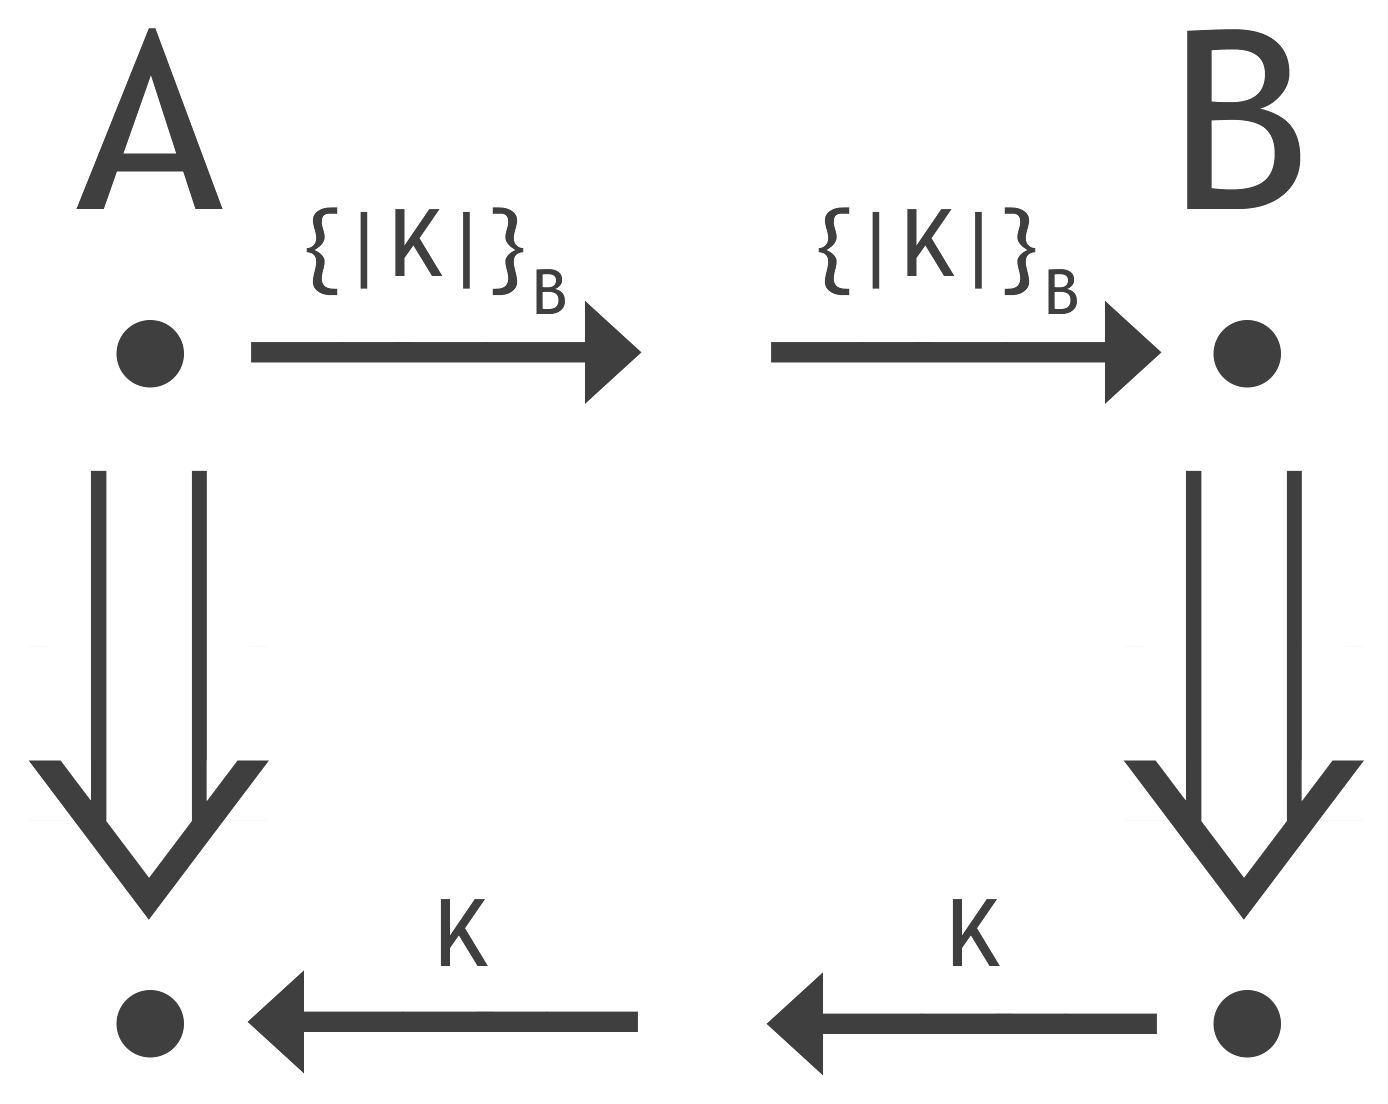
\includegraphics[width=0.5\textwidth]{half-duplex}
			\caption{
				A visual representation of the half-duplex protocol modeled in strand space
				\label{fig:half-duplex}
			}
		\end{figure}

		The geometric logic rules that model this protocol were generated
		manually by direct translation into geometric logic. Ideally, the
		process of generating geometric logic formul{\ae} from protocols should
		be done automatically.

	\subsection{The Results}

		The chase was run on the logic representation of the half-duplex protocol.
		A single model was returned during the execution of the algorithm,
		which was manually stopped before natural completion. This model,
		visualized in Figure \ref{fig:half-duplexCompleted}, like all models
		returned by the chase, satisfies the input theory, and belongs to a set
		of jointly minimal models for the theory.

		\begin{figure}[h]
			\centering
			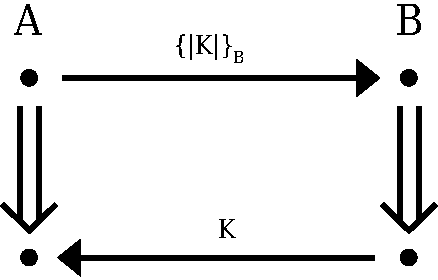
\includegraphics[width=0.5\textwidth]{half-duplexCompleted}
			\caption{
				A visual representation of the discovered run of the half-duplex protocol
				\label{fig:half-duplexCompleted}
			}
		\end{figure}

		The returned model denotes a run of the protocol which contains no
		adversary strands and is a correct execution of the protocol.

\section{Haskell Chase Implementation}
\label{sec:implementation}

	The goal of the implementation of the chase is to deterministically find
	all possible outcomes of the chase. It does this by forking and taking all
	paths when encountering a disjunct rather than nondeterministically
	choosing one disjunct to satisfy.

	The results from the attempts to satisfy each disjunct are returned as a
	list. The returned list will not contain an entry for runs that return no
	model, and will merge lists returned from runs that themselves encountered
	a disjunct. The lazy evaluation of Haskell allows a user to access members
	of the returned list even though some chase runs have not returned a value.

	Appendix \ref{sec:appendixChase} contains the chase-running portions of the
	implementation.

	\subsection{Operation}

		The first step of the chase implementation is to make sure that each
		formula of the given theory can be represented as a geometric logic
		formula. If a formula $\varphi$ can not be coerced to a geometric logic
		formula, the implementation tries to coerce it into one by applying the
		following rules recursively:

		\begin{align*}
		\neg\alpha \wedge \neg\beta         \quad & \mapsto \quad \alpha \vee \beta        \\
		\neg\alpha \vee \neg\beta           \quad & \mapsto \quad \alpha \wedge \beta      \\
		\neg\neg\alpha                      \quad & \mapsto \quad \alpha                   \\
		\neg\alpha \to \beta                \quad & \mapsto \quad \alpha \vee \beta        \\
		\alpha \to \neg\beta                \quad & \mapsto \quad \alpha \wedge \beta      \\
		\neg(\forall\ \vec{x} : \neg\alpha) \quad & \mapsto \quad \exists\ \vec{x} : \alpha
		\end{align*}

		All other constructs are preserved. If this transformed formula is still
		not in positive existential form, an error is thrown.

		The chase function then sorts the input formul{\ae} by the number of
		disjunctions on the right side of the implication. It allows branches to
		terminate without growing to an unnecessarily (and possibly infinitely)
		large size. This step will cause each branch of the algorithm to finish in
		less time, as they are likely to halt before branching yet again. The
		formul{\ae} are not sorted purely by absolute number of disjunctions on the
		right side, but by whether there are zero, one, or many disjunctions. This
		is done to avoid unnecessary re-ordering for no gain because formul{\ae}
		with no disjunctions or only a single disjunct on the right side are more
		likely to cause a branch to stop growing than one with many disjunctions.
		Likewise, formul{\ae} with zero disjunctions are more likely to cause a
		branch to halt than those with one or more disjunctions. A secondary sort
		also occurs within these classifications that orders formul{\ae} by the
		number of variables to reduce the number of bindings generated.

		Once the input formul{\ae} are sorted, the {\tt chase} function begins
		processing a \emph{pending} list, which is initially populated with a
		single model that has an empty domain and no facts.

		For each \emph{pending} model, each formula is evaluated to see if it holds
		in the model for all environments. If an environment is found that does not
		satisfy the model, the model and environment in which the formula did not
		hold is passed to the {\tt satisfy} function, along with the formula that needs
		to be satisfied. The list of models returned from {\tt satisfy} is merged into
		the \emph{pending} list, and the result of running {\tt chase} on the new
		\emph{pending} list is returned. If, however, the model holds for all
		formul{\ae} in the theory and all possible associated environments, it is
		concatenated with the result of running the chase on the rest of the models
		in the \emph{pending} list and returned.

		The {\tt satisfy} function performs a pattern match on the type of formula
		given. Assuming {\tt satisfy} is given a model $\mathbb{M}$, an environment
		$\lambda$, and a formula $\varphi$, {\tt satisfy} will behave as outlined
		in the following algorithm.

		~\\

		\begin{algorithm}[H]
		\DontPrintSemicolon
		\TitleOfAlgo{satisfy :: Model $\to$ Environment $\to$ Sentence $\to$ [Model]}
		return \Switch{$\varphi$}{
			\lCase{$\top$}{return $\{ \mathbb{M} \}$} \;
			\lCase{$\bot$}{return $\emptyset$} \;
			\lCase{$x=y$}{return $\{ quotient(\mathbb{M}) \}$} \;
			\lCase{$\alpha \vee \beta$}{return $satisfy(\alpha) \cup satisfy(\beta)$} \;
			\Case{$\alpha \wedge \beta$}{
				let $r = \emptyset$ \;
				\ForAll{models $m \in satisfy(\alpha)$}{
					redefine $r$ as $r \cup satisfy(\beta)$ \;
				}
				return $r$ \;
			}
			\Case{$\alpha \to \beta$}{
				\lIf{$\mathbb{M}_\lambda \models \alpha$}{return $satisfy(\beta)$ \;}
				\lElse{return $\emptyset$ \;}
			}
			\Case{$R(\vec x)$}{
				define a model $\mathbb{N}$ where $|\mathbb{N}| = |\mathbb{M}| \cup \omega$ and $\omega \not\in |\mathbb{N}|$ to $|\mathbb{N}|$ \;
				\lForEach{$P_\mathbb{M}$}{$P_\mathbb{N} = P_\mathbb{M}$ \;}
				\ForAll{$v \in \vec x$}{
					\lIf{$v \not\in \lambda$}{
						redefine $\lambda$ as $\lambda_{v \mapsto \omega}$ \;
					}
				}
				define $R_{\mathbb{N}}$ as $R_{\mathbb{M}}(\lambda(x_0) \ldots \lambda(x_n))$ \;
				return $\{ \mathbb{N} \}$ \;
			}
			\Case{$\exists\ \vec x : \alpha$}{
				\lIf{$\vec x = \emptyset$}{ return $satisfy(\alpha)$ } \;
				\eIf{$|\mathbb{M}| \ne \emptyset$ and $\exists\ v' \in |\mathbb{M}|$ such that $\lambda' = \lambda_{x_0 \mapsto v'}$ and $\mathbb{M} \models_{\lambda'} \alpha$}{
					return $\{ \mathbb{M} \}$ \;
				}{
					define a model $\mathbb{N}$ where $|\mathbb{N}| = |\mathbb{M}| \cup \omega$ and $\omega \not\in |\mathbb{N}|$ to $|\mathbb{N}|$ \;
					\lForEach{$R_\mathbb{M}$}{$R_\mathbb{N} = R_\mathbb{M}$ \;}
					define $\kappa = \lambda_{x_0 \mapsto \omega}$ \;
					using model $\mathbb{N}$ and environment $\kappa$, return $satisfy(\exists\ \{x_1 \ldots x_n\} : \alpha)$ \;
				}
			}
		}
		\end{algorithm}

		\textbf{TODO: write $quotient$ algorithm and possibly move these to an appendix}

	\subsection{Input Format}

		Input to the program must be in a form parsable by the context-free
		grammar seen in Appendix \ref{sec:appendixParser}. The expected input
		is essentially a newline-separated list of ASCII representations of
		geometric formul{\ae}. Terminals are denoted by a {\tt monospace style}
		and nonterminals are denoted by an $oblique\ style$. The Greek letter
		$\varepsilon$ matches a zero-length list of tokens. Patterns that match
		non-literal terminals are defined in the table in Appendix
		\ref{sec:appendixLexer}.

		Comments are removed at the lexical analysis step and have no effect on
		the input to the parser. Single-line comments begin with either a hash
		({\tt \#}) or double-dash ({\tt --}). Multi-line comments begin with
		{\tt /*} and are terminated by {\tt */}.

	\subsection{Options}

		Help on the usage of the chase implementation can be found by passing
		the executable output by Haskell the {\tt --help} or {\tt -?} options.

		When no options are given to the executable, it expects input from
		stdin and outputs models in a human-readable format to stdout. To take
		input from a file instead, pass the executable the {\tt -i} or {\tt
		--input} option followed by the filename.

		To output models to numbered files in a directory, pass the {\tt -o} or
		{\tt --output} option along with an optional directory name. The given
		directory does not have to exist. If the output directory is omitted,
		it defaults to ``{\tt ./models}".

		Using the {\tt -o} or {\tt --output} options will change the selection
		for output format to a machine-readable format. To switch output formats
		at any time, pass the {\tt -h} or {\tt -m} flags for human-readable and
		machine-readable formats respectively.


	\subsection{Future Considerations}

		This section details areas of possible improvement/development.

		\subsubsection{Better Data Structures}

			Some less-than-optimal data structures are being used to hold data
			that should really be in a Data.Map or Data.Set. One such example
			of this is with the truth table holding the relation information of
			a model. This truth table should be implemented as a Data.Map.
			Environments are currently a list of tuples, but should really be a
			Data.Map. Instead of Domains being a list of DomainMember, it
			would be better if a Domain was a Data.Set.

		\subsubsection{Broader Use of the Maybe Monad}

			In several helper functions, the program's execution is halted and
			an error is output when the function receives certain invalid
			inputs. These functions should take advantage of the Maybe Monad
			and return {\tt Maybe a} where {\tt a} is the type they currently
			return. One particular example of this is the {\tt pef} function.
			When {\tt pef} takes a formula as input that can not be converted
			to positive-existential form, it causes the program to produce an
			error and exit. Instead, {\tt pef} should return {\tt Maybe
			Formula} and the places where it is used should handle the error
			condition however they choose.

		\subsubsection{Binding Search Approach for Satisfaction Checking}

			When checking if a model with 30 domain members and 60 facts holds
			for a formula with 5 universally quantified variables (a reasonable
			real-life usage example), $30^5$ or $24,300,000$ bindings will have
			to be generated, and the formula will be checked under each one.
			But by limiting the checked bindings to only those that can produce
			facts that exist in the model from the atomics in the formula, only
			the 60 facts will have to be checked in the worst case, and only 1
			in the best. In practical use, this should dramatically reduce the
			running time of theories that produce finite results.

		\subsubsection{Avoid Isomorphic Model Generation}

			By taking different paths to arrive at the same model, the chase
			often creates equivalent models that satisfy its given theory.
			These duplicate models are already being filtered from the output.
			However, another problem exists when the chase returns isomorphic
			models. Given two models, it is very computationally expensive to
			determine if there exists an isomorphism between them. If a fast
			method of determining if two models are isomorphic is found,
			including an implementation of it would provide more valuable
			results to the user.

		\subsubsection{Improve Efficiency}

			The main goals of this project were to write a correct chase
			implementation and apply it in a real-world situation. While
			reasonable and obvious optimizations were made, there is still
			plenty of room for optimization.

			In \cite{Harrison09} Harrison's \emph{Practical Logic and Automated
			Reasoning}, Harrison mentions a large number of formula rewriting
			and simplification algorithms, many of which are already
			implemented in the Helpers module. Those functions that are
			written, however, are not currently being used by the chase
			functions, and there are surely other functions that Harrison
			mentions that have not yet been written.

			One specific example of a function that \cite{Harrison09} Harrison
			mentions on pages 141 to 144 is {\tt pullQuants}, which pulls all
			quantifiers in a formula to the outside. This results in a formula
			with no conjunctions or disjunctions of quantified subformul{\ae}.
			This function is implemented, but a function that does exactly the
			opposite of this will help speed up satisfaction checking when
			using the traditional looping method. This will minimize the number
			of times bindings need to be generated for all permutations of the
			current model's domain because the number of quantified variables
			will be reduced.

		\subsubsection{Tracing}

			Currently, Debug.Trace is being used to output real-time status for
			ease of debugging. This output is helpful to both developers of
			the chase implementation and theories that will be given as input.
			Unfortunately, all of the output can really slow down a chase run
			of a simple theory. Currently, the only way to disable tracing is
			to replace the definition \[trace = Debug.Trace.trace\] with
			\[trace\ x = id\]

			A flag is already being read in from the command line as {\tt -d}
			and stored in the options record under {\tt optDebug}. When this
			flag is found, a callback function is being invoked in the Main
			module. Someone who implements this enhancement would need to be
			able to alter the behaviour of the Chase module's $trace$ function
			from a function within the Main module.  Ideally, a better
			debugging output method will be found and Debug.Trace.trace will no
			longer need to be used in what is otherwise production-ready code.


\singlespacing

%\section{For later reference:}
%	\begin{figure}[graphics_test]
%		\begin{center}
%			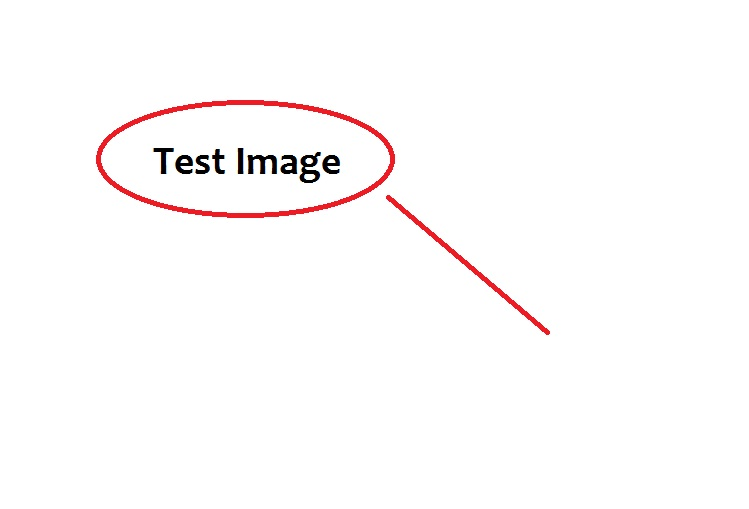
\includegraphics[width=0.8\textwidth]{pic1.jpg}
%		\end{center}
%		\caption[Caption in List of Figures]{Caption in report}
%	\end{figure}


\appendix
	\section{Table of Syntax}
	\begin{tabular}{|r|l|}
		\hline
		\textbf{syntax}                  &  \textbf{definition}                                                     \\
		\hline
		$f^{-1}$                         &  the inverse function of $f$                                             \\
		\hline
		$R[a_0,a_1,a_2]$                 &  a \emph{relation} of: relation symbol $R$, arity $3$, and tuple $\langle a_0,a_1,a_2 \rangle$  \\
		$\top$                           &  a \emph{tautological formula}; one that will always hold                \\
		$\bot$                           &  a \emph{contradictory formula}; one that will never hold                \\
		$\rho = \tau$                    &  given assumed environment $\lambda$, $\lambda(\rho) = \lambda(\tau)$    \\
		$\neg \alpha$                    &  $\alpha$ does not hold                                                  \\
		$\alpha \wedge \beta$            &  both $\alpha$ and $\beta$ hold                                          \\
		$\alpha \vee \beta$              &  either $\alpha$ or $\beta$ hold                                         \\
		$\alpha \to \beta$               &  either $\alpha$ does not hold or $\beta$ holds                          \\
		$\forall x : \alpha$             &  for each member of the domain as $x$, $\alpha$ holds                    \\
		$\forall \vec{x} : \alpha$       &  for each $x_i \in x$, $\forall x_i : \alpha$ holds                      \\
		$\exists x : \alpha$             &  for at least one member of the domain as $x$, $\alpha$ holds            \\
		$\exists \vec{x} : \alpha$       &  for each $x_i \in x$, $\exists x_i : \alpha$ holds                      \\
		\hline
		$\lambda[x \mapsto y]$           &  the environment $\lambda$ with variable $x$ mapped to domain member $y$ \\
		\hline
		$\mathbb{M} \models_l \sigma$    &  $\mathbb{M}$ \emph{is a model of} $\sigma$ under environment $l$        \\
		$\mathbb{M} \models \sigma$      &  $\mathbb{M} \models_l \sigma$ given any environment $l$                 \\
		$\mathbb{M} \models_l \Sigma$    &  for each $\sigma \in \Sigma$, $\mathbb{M} \models_l \sigma$             \\
		$\mathbb{M} \models \Sigma$      &  for each $\sigma \in \Sigma$, $\mathbb{M} \models \sigma$               \\
		\hline
		$\Sigma \models \sigma$          &  $\Sigma$ \emph{entails} $\sigma$                                        \\
		\hline
		$\mathbb{M} \preceq \mathbb{N}$  &  there exists a \emph{homomorphism} $h : |\mathbb{M}| \to |\mathbb{N}|$  \\
		$\mathbb{M} \simeq \mathbb{N}$   &  $\mathbb{M}$ and $\mathbb{N}$ are \emph{homomorphically equivalent}     \\
		\hline
	\end{tabular}

	\section{Chase code}
\label{sec:appendix_chase}

	\textbf{TODO: make the long lines short so they fit}
	{\scriptsize
		\lstset{
			language=Haskell,
			numbers=left,
			columns=fixed,
			tabsize=3,
		}
		\lstinputlisting{../chase.hs}
	}



\addcontentsline{toc}{section}{References}
\begin{thebibliography}{9999}

\bibitem{AC}
	A~Cottrell, \textsl{Word Processors: Stupid and Inefficient},\\
	\mbox{} \hfill \url{www.ecn.wfu.edu/\~cottrell/wp.html}

\end{thebibliography}



\end{document}
